
\documentclass[8pt]{beamer}

\usepackage[english]{babel}
\usepackage[utf8]{inputenc}
\usepackage{pdfpages}
\usepackage{color}
\usepackage{graphicx, import}
\usepackage{amsmath}
\usepackage{amssymb}
\usepackage{physics} % norm
\usepackage{tikz}
\usepackage{pgfplots}
\usepackage{tabularx}
\usepackage[numbers, square]{natbib}
\usepackage{mathtools}
\usepackage{caption} % change style of figure 
\usepackage{subcaption}
\usepackage{booktabs}

\usetikzlibrary{positioning, fit, patterns, snakes, chains, arrows, decorations.markings}
%\tikzexternalize[prefix=out/figures/]
\newcolumntype{Y}{>{\centering\arraybackslash}X} % centered equidistant columns

\bibliographystyle{plainnat}
\usetheme{metropolis}
\setbeamertemplate{frame footer}{\insertshortauthor\hfill\insertshortinstitute}
\setbeamercolor{footline}{fg=gray}


\title[]{Weakly Supervised 2D to 3D Lifting of Human Poses}
\author[Nikolas Klug]{Nikolas Klug}
\institute[University of Augsburg]{University of Augsburg}
\date{22 August 2019}


\begin{document}
	{
	\setbeamertemplate{footline}{}
	\begin{frame}
		\titlepage
	\end{frame}
	}
	\addtocounter{framenumber}{-1}

	\begin{frame}
		\begin{figure}
			\vspace{1cm}
			\begin{tikzpicture}
				[
				start chain = A going right,
				txt/.style = {text height=2ex, text depth=0.25ex, font=\sffamily\bfseries\Large,
					on chain},
				every edge/.append style = {draw, -stealth'}
				]
					\node [txt] (weakly) [] {Weakly Supervised};
					{\visible<3->{\draw
					[thick,
					decoration={brace, mirror, raise=0.2cm},
					decorate,
					align=center
					] 
					(weakly.west) -- (weakly.east) node [pos=0.5,anchor=north,yshift=-0.55cm] {using a \\ Generative Adversarial Network \\ -- no ground truth data required};}}
					\node [txt] [right=.2 of weakly] (2Dto3D) [] {2D to 3D Lifting of Human Poses};
					{\visible<2->{\draw 
					[thick,
					decoration={brace, mirror, raise=0.2cm},
					decorate,
					] 
					(2Dto3D.west) -- (2Dto3D.east) node [pos=0.5,anchor=north,yshift=-0.55cm] {};}}
					\visible<2->{
						\node [below left=2cm and -2cm of 2Dto3D] (2Dpose) {\scalebox{-1}[1]{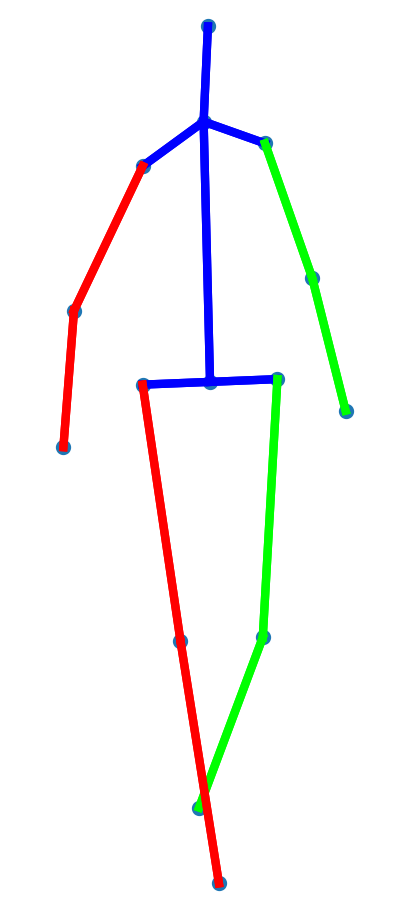
\includegraphics[height=3.2cm]{figures/2D_pose_426411.png}}};
						\node [below right=2cm and -3cm of 2Dto3D] (3Dpose) {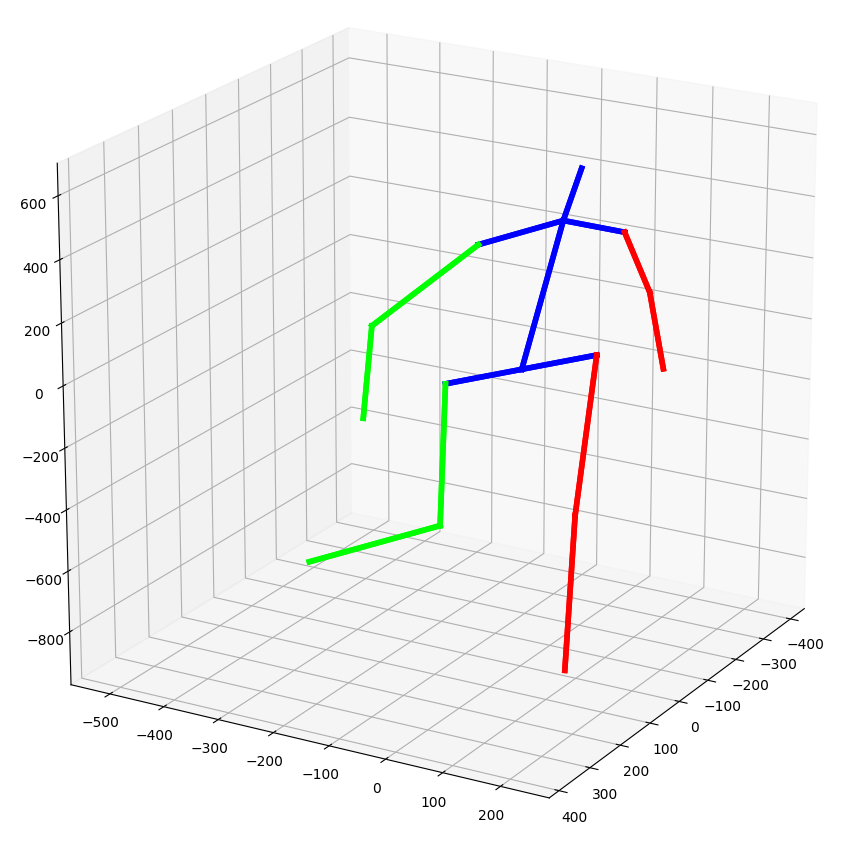
\includegraphics[height=3.2cm]{figures/3D_pose_426411.png}};
						\node [below= 0cm of 2Dpose] (2Dtext) [] {2D pose};
						\node [below= 0cm of 3Dpose] (3Dtext) [] {3D pose};
						\draw [dashed, decoration={markings,mark=at position 1 with
							{\arrow[scale=2,>=stealth]{>}}},postaction={decorate}] (2Dpose.east) -- (3Dpose.west);
						\node[fit=(2Dpose)(3Dpose)(2Dtext)(3Dtext)] (poses) {};
						\draw [decoration={markings,mark=at position 1 with
							{\arrow[scale=2,>=stealth]{>}}},postaction={decorate}] ([yshift=-0.2cm]2Dto3D.south) -- ([yshift=-1.5cm]2Dto3D.south);
					}
			\end{tikzpicture}
		\end{figure}
	\end{frame}

	\begin{frame}{Source}
		\textbf{Can 3D Pose be Learned from 2D Projections Alone?}\linebreak
		\begin{footnotesize}
			Dylan Drover, Rohith MV, Ching-Hang Chen, Amit Agrawal, Ambrish Tyagi, and Cong Phuoc Huynh.\linebreak
			In Computer Vision -- ECCV 2018 Workshops, Pages 78-94, 2019. Springer International Publishing.
		\end{footnotesize}
	\end{frame}

	\begin{frame}{Why?}
		\begin{itemize}
			\item Very good 2D keypoint detectors out there: Stacked Hourglass, OpenPose etc.
			\item Massive amount of 2D images/videos available
			\item Acquiring 3D ground truth data is cumbersome and expensive
		\end{itemize}
	\end{frame}

	\begin{frame}{Underlying heuristic}
		\textbf{If a random 2D projection of a 3D pose looks realistic, the 3D pose is realistic.}
	\end{frame}

	\begin{frame}{How It Works}
		\begin{figure}
			\centering
			\makebox[\textwidth][c]{
				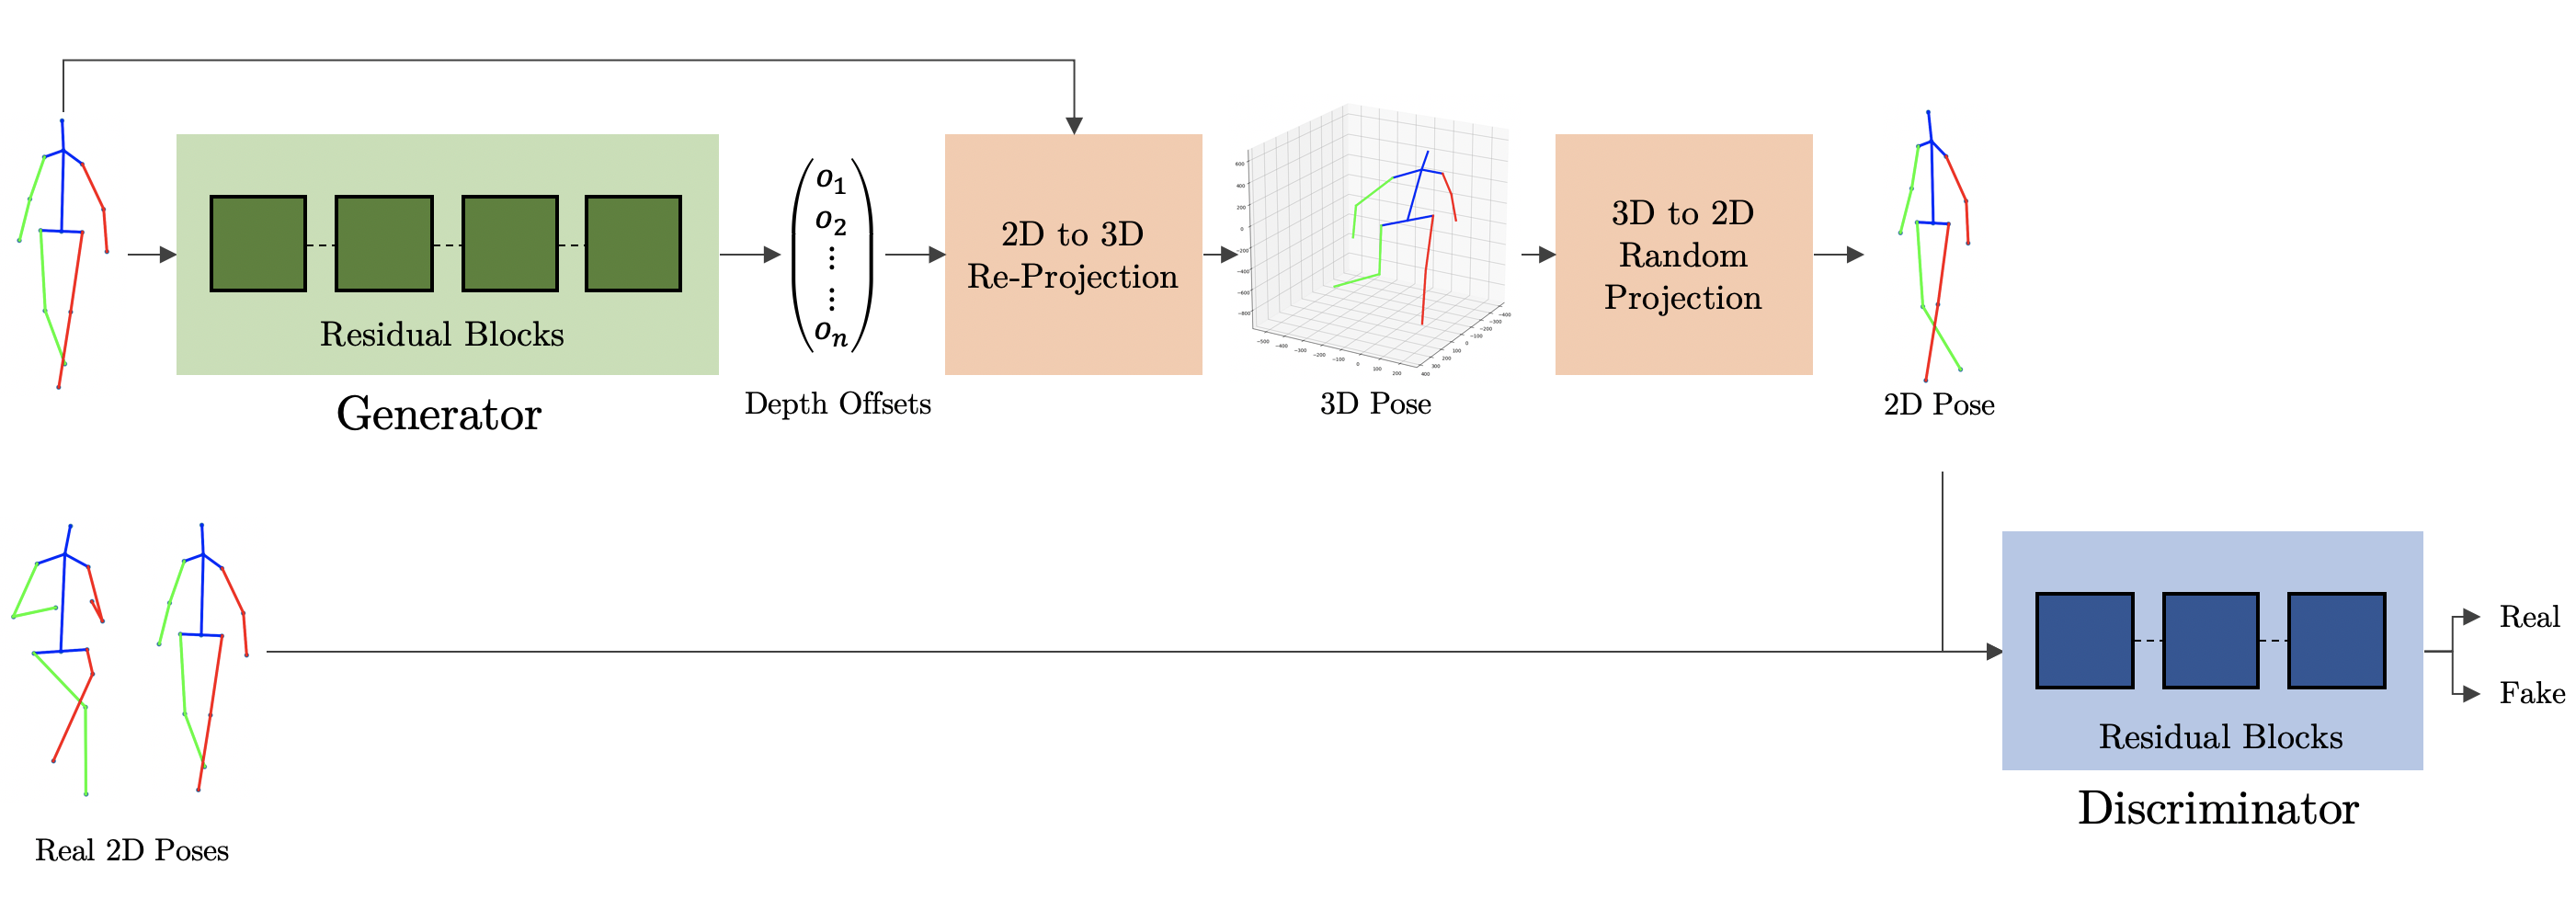
\includegraphics[width=1.1\textwidth]{figures/system.png}
			}                
		\end{figure}
	\end{frame}

	\begin{frame}{Results}
		\begin{table}
			\centering
			\begin{tabularx}{\textwidth}{l *{8}{Y}}
				\toprule
				Method & Direct. & Discuss & Eat & Greet & Phone & Pose & Purchase & Sit \\
				\midrule
				w/o rotation & 48.8 & 51.5 & 41.5 & 57.7 & 49.4 & 54.3 & 48.8 & 50.0 \\
				w/ rotation & 36.3 & 35.5 & 35.6 & 42.6 & 34.8 & 44.1 & 45.2 & 36.3 \\
				\bottomrule
				\toprule
				Method & SitDown & Smoke & TPhoto & Wait & Walk & WDog & WTog. & \textbf{Avg.}\\
				\midrule
				w/o rotation & 64.3 & 51.9 & 64.6 & 57.1 & 54.3 & 57.9 & 53.2 & \textbf{54.8} \\
				w/ rotation  & 51.9 & 41.9 & 50.8 & 43.0 & 38.5 & 49.6 & 40.8 & \textbf{41.0} \\
				\bottomrule
			\end{tabularx}
		\caption{Mean Per Joint Position Errors for synthetic poses from the Human3.6M dataset with and without rotation to fit the estimated poses to the ground truth data. The MPJPEs are given in millimeters.}
		\end{table}
	\end{frame}
	
	\begin{frame}{Introduction of Limb Loss}
		Punishes the generator if it produces 3D poses with symmetric limbs of different lengths
		\vspace{2em}
		\begin{equation*}
			loss_{limb} = \frac{1}{|S|}\sum_{((u_1, v_1), (u_2, v_2)) \in S} \bigl\lvert \norm{u_1 - v_1}_2 - \norm{u_2 - v_2}_2 \bigr\rvert
		\end{equation*}		
	\end{frame}

	\begin{frame}{Results for Limb Loss}
		\begin{table}[bt]	
			\centering
			\begin{tabularx}{\textwidth}{l *{8}{Y}}
				\toprule
				Method & Direct. & Discuss & Eat & Greet & Phone & Pose & Purchase & Sit \\
				\midrule
				$loss_G$ & 48.2 & 52.9 & 47.4 & 58.7 & 54.3 & 57.6 & 51.7 & 52.5\\
				$loss_{G, limb}$ & 42.9 & 51.6 & 41.9 & 55.0 & 49.2 & 51.6 & 51.1 & 45.9 \\
				\bottomrule
				\toprule
				Method & SitDown & Smoke & TPhoto & Wait & Walk & WDog & WTog. & \textbf{Avg.}\\
				\midrule
				$loss_G$ & 64.3 & 51.9 & 64.6 & 57.1 & 54.3 & 57.9 & 53.2 & \textbf{54.8} \\
				$loss_{G, limb}$ & 61.0 & 47.0 & 61.4 & 54.4 & 45.7 & 56.7 & 48.1 & \textbf{50.7} \\
				\bottomrule
			\end{tabularx}
			\caption{
				Comparison of the MPJPEs with standard and modified loss for the Human3.6M dataset without rotation. The MPJPEs are given in millimeters.
			}
			\label{tbl:results-limb-loss}
		\end{table}
	\end{frame}

	\begin{frame}{Analysis of the Effects of Pose Normalization}
		The 2D poses are normalized in scale and position before being fed to the generator.
		\begin{figure}
			\begin{subfigure}[]{.45\textwidth}
				\centering
				\begin{tikzpicture}[trim axis left]
					\begin{axis}[
					tiny,
					width=1.25\textwidth,
					xlabel={$dx$ [m]},
					%			axis lines = middle,
					y label style={at={(axis description cs:0.1,1.1)},rotate=-90,anchor=north},
					ylabel={MPJPE [mm]},
					grid=both,
					enlarge x limits = false,
					grid style={draw=gray!50},
					minor tick num = 1,
					tick style={draw=gray!50},
					xtick={-100,-50,0,50,100},
					extra x ticks={0},
					scaled x ticks = false,
					no markers,
					every axis plot/.append style={}
					]
					\addplot table [x=a, y=b, col sep=comma] {figures/plot_e_03_07_original_x_shift.csv};
					\addplot table [x=a, y=b, col sep=comma] {figures/plot_theoretical_x_shift_scaled.csv};
					\end{axis}
					\end{tikzpicture}
			\end{subfigure}\hfill
			\begin{subfigure}[]{.45\textwidth}
				\centering
				\begin{tikzpicture}[trim axis left]
				\begin{axis}[
				tiny,
				width=1.25\textwidth,
				xlabel={$dx$ [m]},
				%			axis lines = middle,
				y label style={at={(axis description cs:0.1,1.1)},rotate=-90,anchor=north},
				ylabel={MPJPE [mm]},
				grid=both,
				enlarge x limits = false,
				grid style={draw=gray!50},
				minor tick num = 1,
				tick style={draw=gray!50},
				xtick={-3,-2,-1,0,1,2,3},
				extra x ticks={0},
				scaled x ticks = false,
				no markers,
				every axis plot/.append style={}
				]
				\addplot +[restrict expr to domain={\coordindex}{180:401}] table [x=a, y=b, col sep=comma] {figures/plot_e_03_07_original_x_shift.csv};
				\addplot +[restrict expr to domain={\coordindex}{180:401}] table [x=a, y=b, col sep=comma] {figures/plot_theoretical_x_shift_scaled.csv};
				\end{axis}
				\end{tikzpicture}
			\end{subfigure}
			\caption{Theoretical (red) and experimental (blue) MPJPEs for different values of $dx$ without rotation.
				The distance between the camera and the poses is approximately 5m.}
		\end{figure}
	\end{frame}

	\begin{frame}{Results for Modified Network}
		\begin{figure}
			\begin{subfigure}[]{.63\textwidth}
				\centering
				\begin{tikzpicture}[trim axis left]
				\begin{axis}[
				tiny,
				width=1.25\textwidth,
				xlabel={$dx$ [m]},
				%			axis lines = middle,
				y label style={at={(axis description cs:0.05,1.07)},rotate=-90,anchor=north},
				ylabel={MPJPE [mm]},
				grid=both,
				enlarge x limits = false,
				grid style={draw=gray!50},
				minor tick num = 1,
				tick style={draw=gray!50},
%				xtick={-3,-2,-1,0,1,2,3},
				extra x ticks={0},
				scaled x ticks = false,
				no markers,
				every axis plot/.append style={}
				]
				\addplot +[restrict expr to domain={\coordindex}{90:491}] table [x=a, y=b, col sep=comma] {figures/plot_e_03_07_original_x_shift.csv};
				\addplot[color=black!60!green] table [x=a, y=b, col sep=comma] {figures/plot_e_01_06_shifted_generator_x_shift.csv};
				\end{axis}
				\end{tikzpicture}
			\end{subfigure}
			\caption{MPJPEs for original (blue) and modified (green) network for different values of $dx$ without rotation.
				The distance between the camera and the poses is approximately 5m.}
		\end{figure}
	\end{frame}
	
	
\end{document}